\documentclass[11pt]{article}
\usepackage[margin=1in]{geometry}
\usepackage{amsmath}
\usepackage[utf8]{inputenc}
\usepackage[T1]{fontenc}
\usepackage{mathpazo}
\usepackage{eulervm}
\usepackage{tabularx}
\usepackage{enumitem}
\usepackage{physics}
\usepackage{hyperref}
\usepackage{xcolor}
\usepackage{graphicx}
\usepackage{caption}
\usepackage{subcaption}
\captionsetup{labelfont=bf,
	justification=centering,
	labelsep=newline, % <<< label and text on different lines
	singlelinecheck=false,
	margin=1em}

\hypersetup{
	colorlinks=true,
	filecolor=blue,
	linkcolor=blue,
	citecolor=blue,
	urlcolor=purple}

\newcommand{\itemspacing}{
	\setlength{\parskip}{0pt}\setlength{\itemsep}{0pt}
}

\usepackage[authoryear]{natbib}
\bibliographystyle{apalike}
\title{\textsc{\Large Coding Project\\}PH 549: Physics of Biological Systems\\}
\author{Vedant Prakash Shenoy (170260028)}
\begin{document}
\maketitle
\section{Overview}
\citet[henceforth referred to as 'the paper']{PhysRevE.76.041907} aims to model microtubule growth using a simple kinetic model. The model makes use of the following processes ((\ref{eq:attach}) Attachment, (\ref{eq:convert}) Conversion, and (\ref{eq:detach}) Detachment):
\begin{equation}
\label{eq:attach}
\begin{split}
\ket{\dots+} &\Rightarrow \ket{\dots++}\hspace{2em} \text{rate }\lambda\\
\ket{\dots-} &\Rightarrow \ket{\dots-+}\hspace{2em} \text{rate }p\lambda\\
\end{split}
\end{equation}
\begin{equation}
\label{eq:convert}
\ket{\dots+\cdots} \Rightarrow \ket{\dots-\cdots}\hspace{2em} \text{rate }1
\end{equation}
\begin{equation}
\label{eq:detach}
\ket{\dots-} \Rightarrow \ket{\dots}\hspace{2em} \text{rate }\mu
\end{equation}
where $+$ and $-$ represent the GTP and GDP monomer units respectively. \\\\
The main results that I have replicated are as follows\footnote{Figures 2 and 3 are cartoons to explain the model and have not been reproduced here}:
\begin{enumerate}
%\itemspacing
\item Microtubule Length as a function of time and the parameters $(\lambda, p, \mu)$. (Figure 1 of the paper)
\item Distribution of the GTP cap length (Figure 4 of the paper)
\item Distribution of GTP islands in the microtubule (Figure 5 of the paper)
\item Phase Diagrams of microtubule growth (Figure 6 of the paper)
\end{enumerate}

I numerically simulated the system using the BKL algorithm \citep[reviewed in, for example,][]{10.3389/fchem.2019.00202}. However no particular scheme was mentioned in the paper.\\

Once the numerical simulation is implemented, replicating Figures 1, 4 and 5 is straightforward (with any minor changes made in the calculations mentioned in the respective Figure captions). However, for Figure~6 in the paper, an alternate approximation was employed, which underestimates the actual phase boundary, which is discussed in Section~\ref{sec:disc}

\section{Figures}
\label{sec:figs}
Figures on top on each page is the original and the bottom figure is the replicated version.

\begin{figure}[!h]
\centering
\begin{subfigure}{\linewidth}
	\centering
	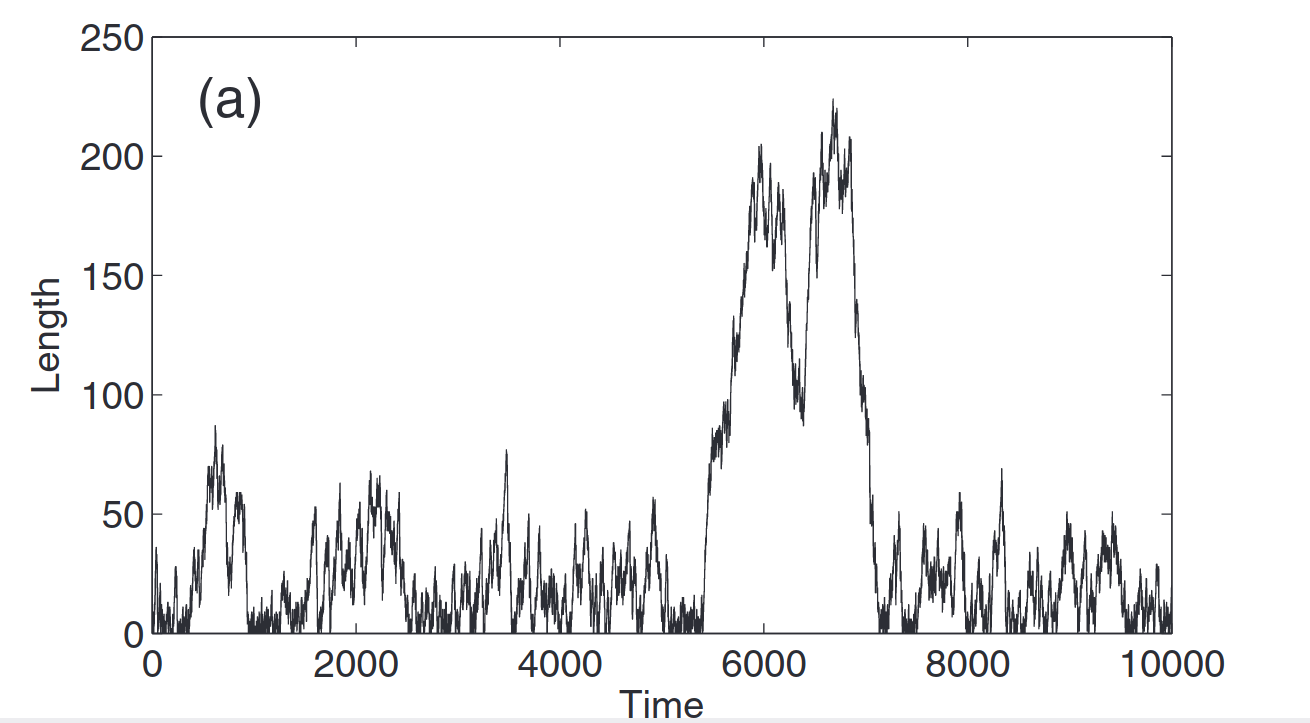
\includegraphics[width=\linewidth]{plots/1a.png}
%	\caption{Original Figure 1a}
\end{subfigure}
\begin{subfigure}{\linewidth}
	\centering
	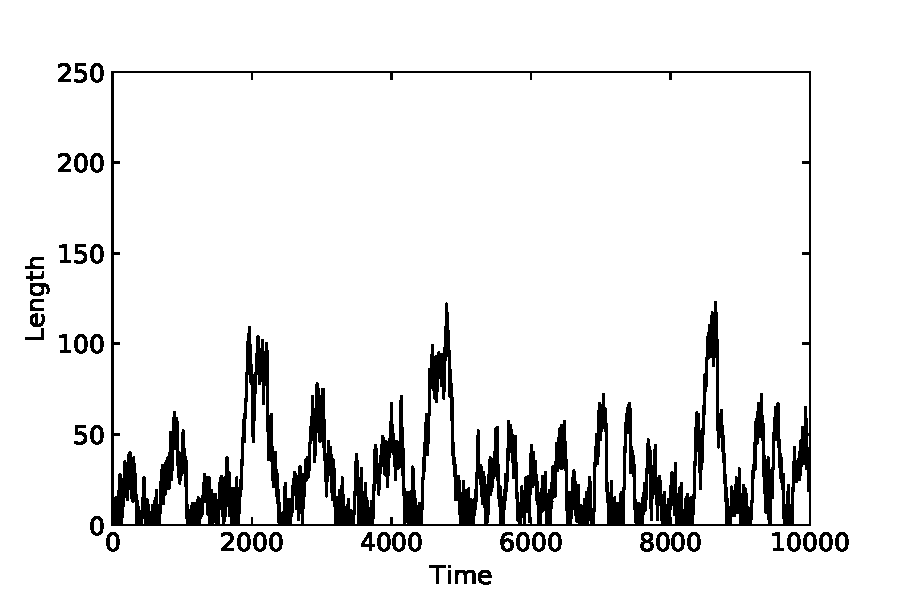
\includegraphics[width=\linewidth]{plots/1a.pdf}
%	\caption{Replicated Figure 1a}
\end{subfigure}
\caption{Microtubule growth for $\lambda=1.4$, $p=1$, $\mu=5$}
\end{figure}

\begin{figure}[!h]
	\centering
	\begin{subfigure}{\linewidth}
		\centering
		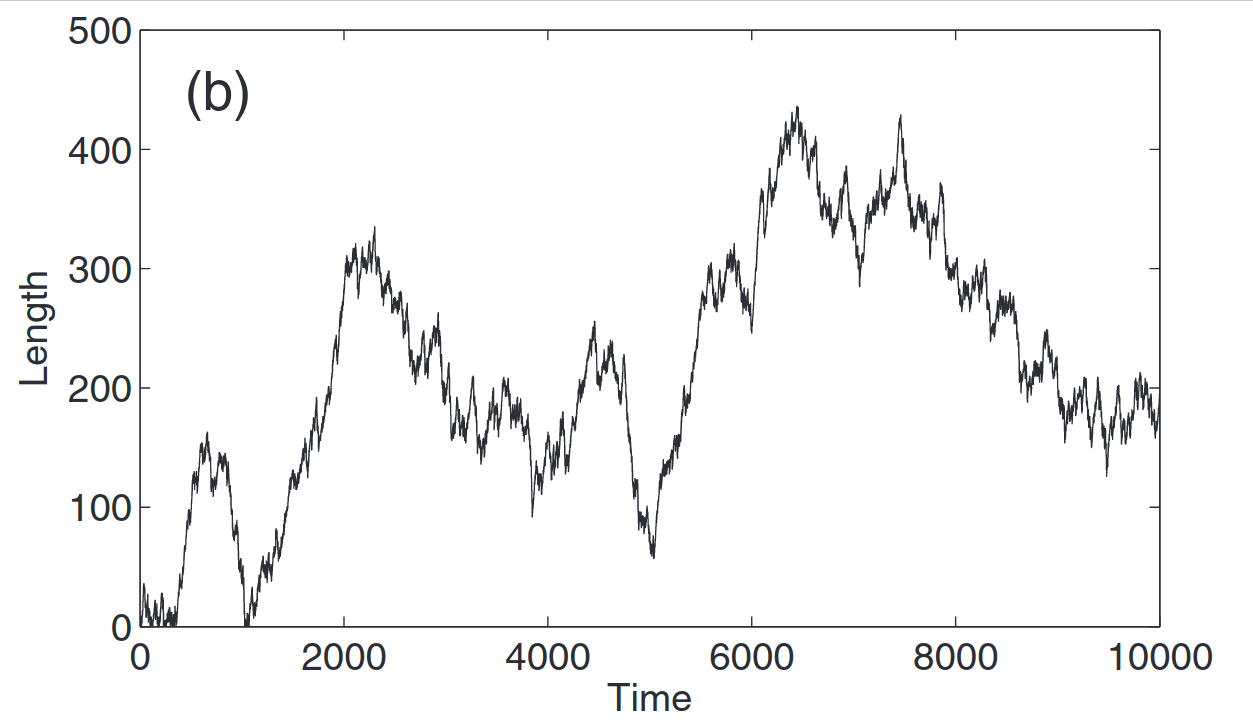
\includegraphics[width=\linewidth]{plots/1b.png}
%		\caption{Original Figure 1b}
	\end{subfigure}
	\begin{subfigure}{\linewidth}
		\centering
		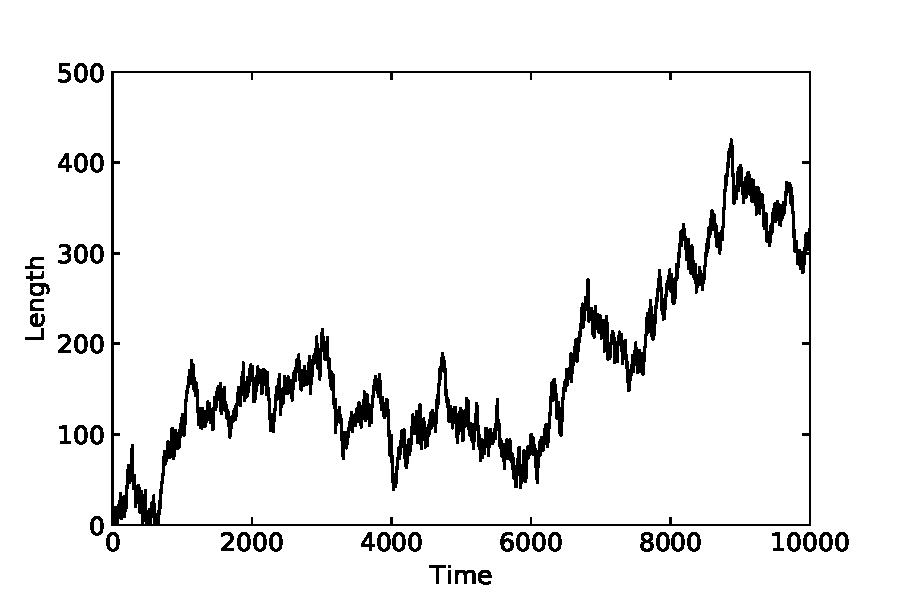
\includegraphics[width=\linewidth]{plots/1b.pdf}
%		\caption{Replicated Figure 1b}
	\end{subfigure}
	\caption{Microtubule growth for $\lambda=1.5$, $p=1$, $\mu=5$}
\end{figure}

\begin{figure}[!h]
	\centering
	\begin{subfigure}{\linewidth}
		\centering
		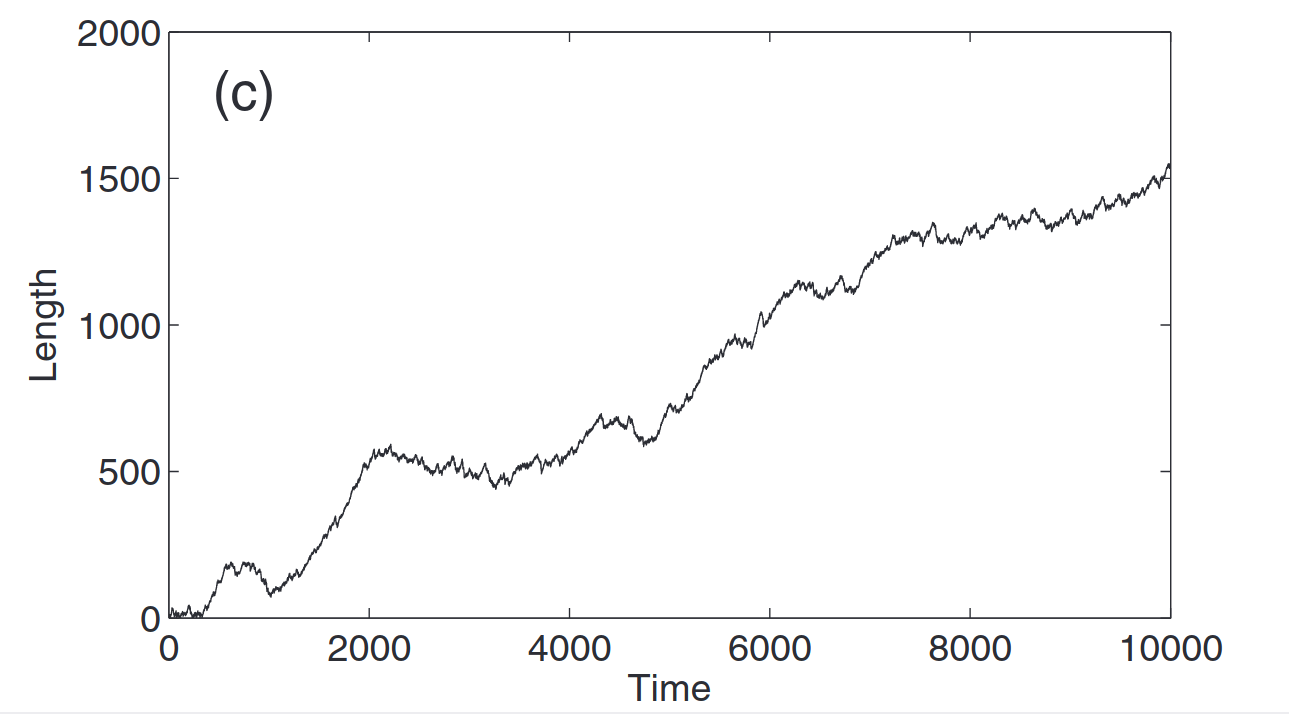
\includegraphics[width=\linewidth]{plots/1c.png}
%		\caption{Original Figure 1c}
	\end{subfigure}
	\begin{subfigure}{\linewidth}
		\centering
		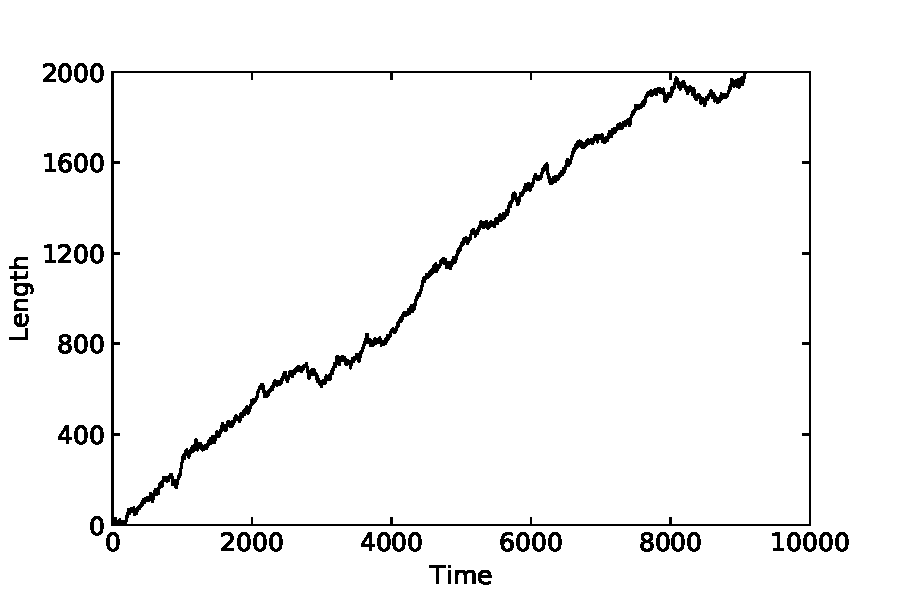
\includegraphics[width=\linewidth]{plots/1c.pdf}
%		\caption{Replicated Figure 1c}
	\end{subfigure}
	\caption{Microtubule growth for $\lambda=1.6$, $p=1$, $\mu=5$}
\end{figure}

\begin{figure}[!h]
	\centering
	\begin{subfigure}{\linewidth}
		\centering
		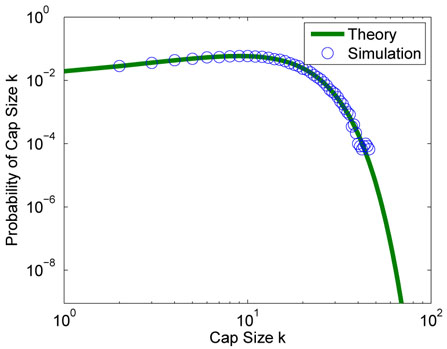
\includegraphics[width=14cm]{plots/4.jpg}
%		\caption{Original Figure 4}
	\end{subfigure}
	\begin{subfigure}{\linewidth}
		\centering
		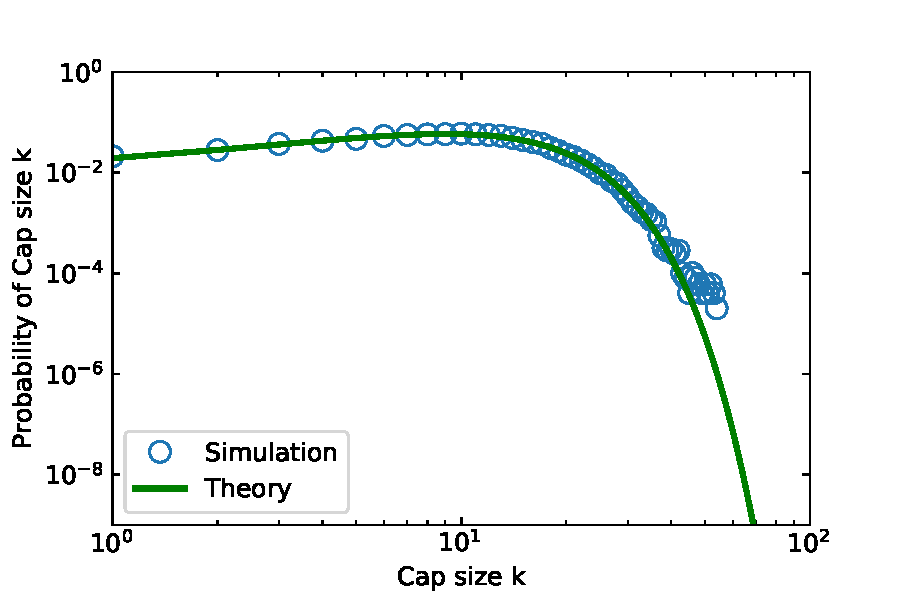
\includegraphics[width=15cm]{plots/4.pdf}
%		\caption{Replicated Figure 4}
	\end{subfigure}
	\caption{Capsize distribution for $\lambda=100$, $p=1$, $\mu=0$}
\end{figure}

\begin{figure}[!h]
	\centering
	\begin{subfigure}{\linewidth}
		\centering
		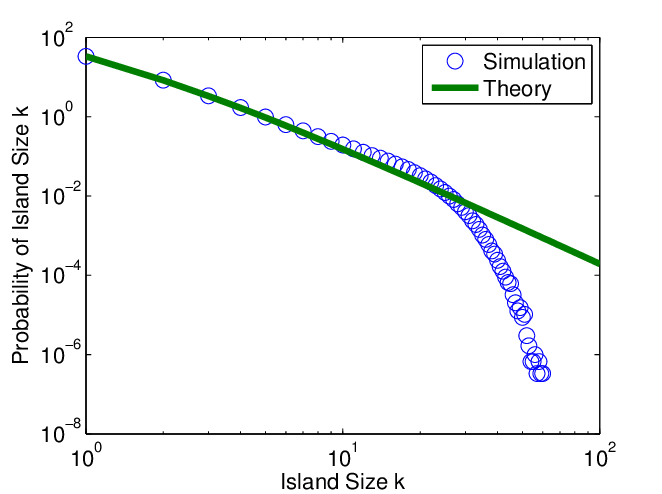
\includegraphics[width=14cm]{plots/5.png}
%		\caption{Original Figure 5}
	\end{subfigure}
	\begin{subfigure}{\linewidth}
		\centering
		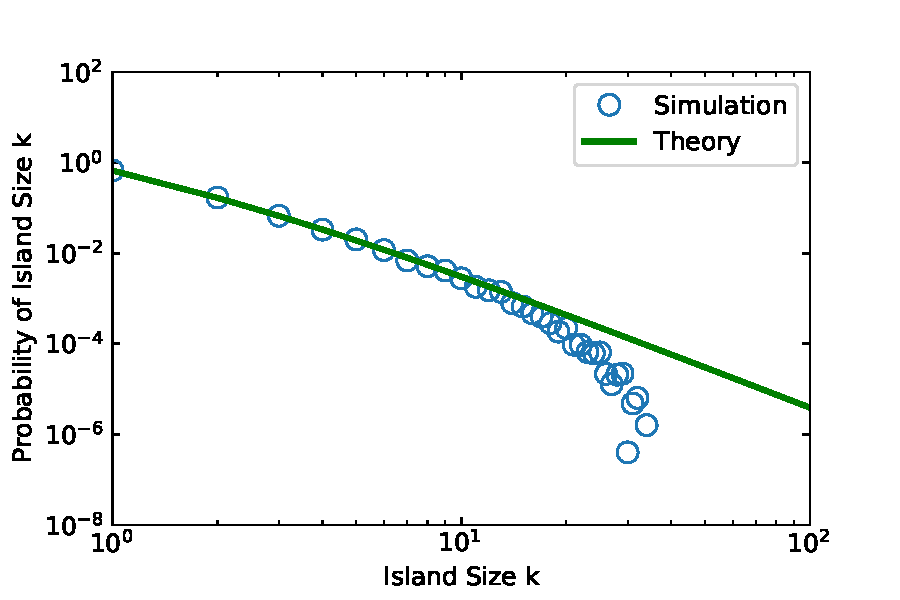
\includegraphics[width=15cm]{plots/5.pdf}
%		\caption{Replicated Figure 5}
	\end{subfigure}
	\caption{Island size distribution for $\lambda=100$, $p=1$, $\mu=0$. Plots differ by a scaling factor in the definition of Island Size}
\end{figure}

\begin{figure}[!h]
	\centering
	\begin{subfigure}{\linewidth}
		\centering
		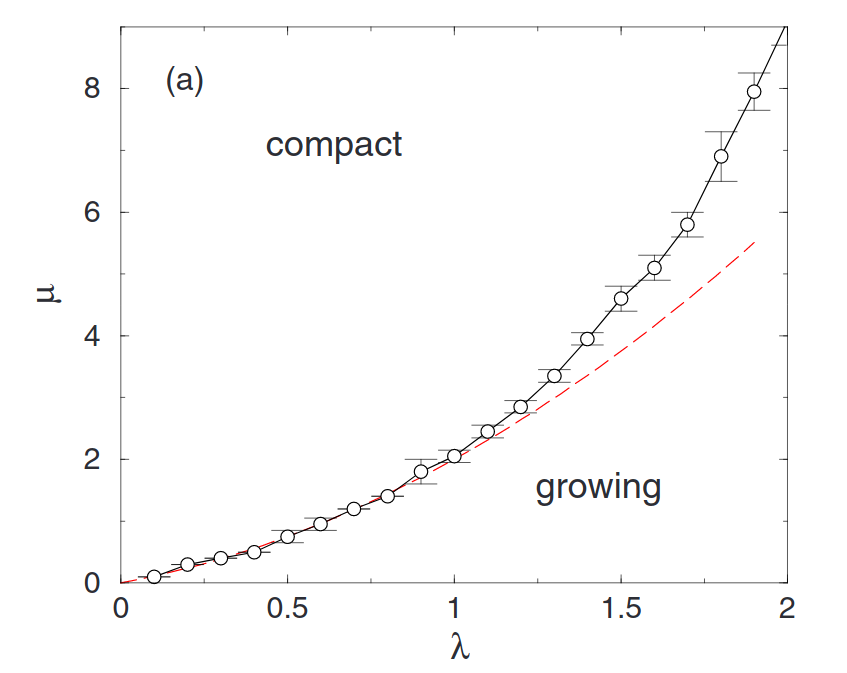
\includegraphics[width=14cm]{plots/6a.png}
%		\caption{Original Figure 6a}
	\end{subfigure}
	\begin{subfigure}{\linewidth}
		\centering
		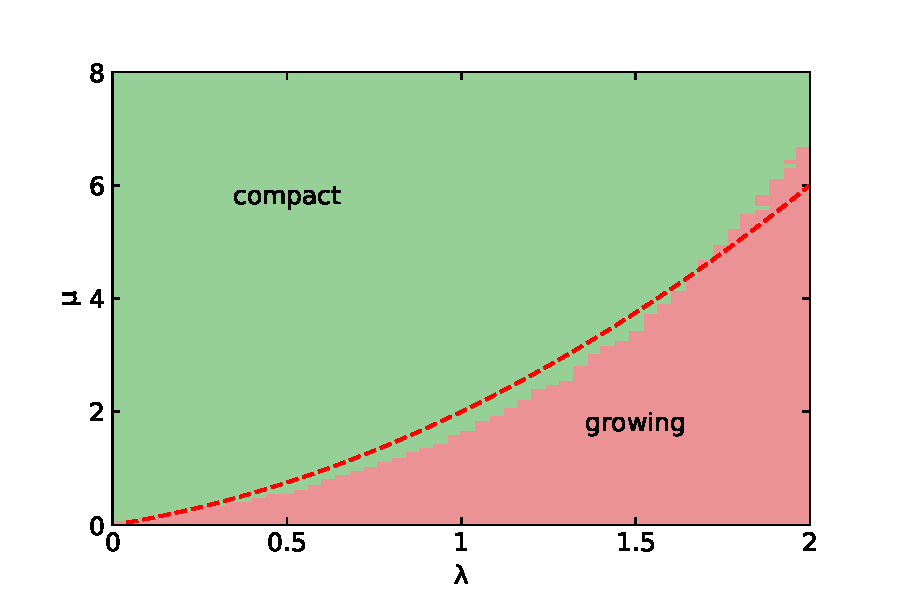
\includegraphics[width=15cm]{plots/6a.pdf}
%		\caption{Replicated Figure 6a}
	\end{subfigure}
	\caption{Phase Diagram for $p=1$}
\end{figure}
\begin{figure}[!h]
	\centering
	\begin{subfigure}{\linewidth}
		\centering
		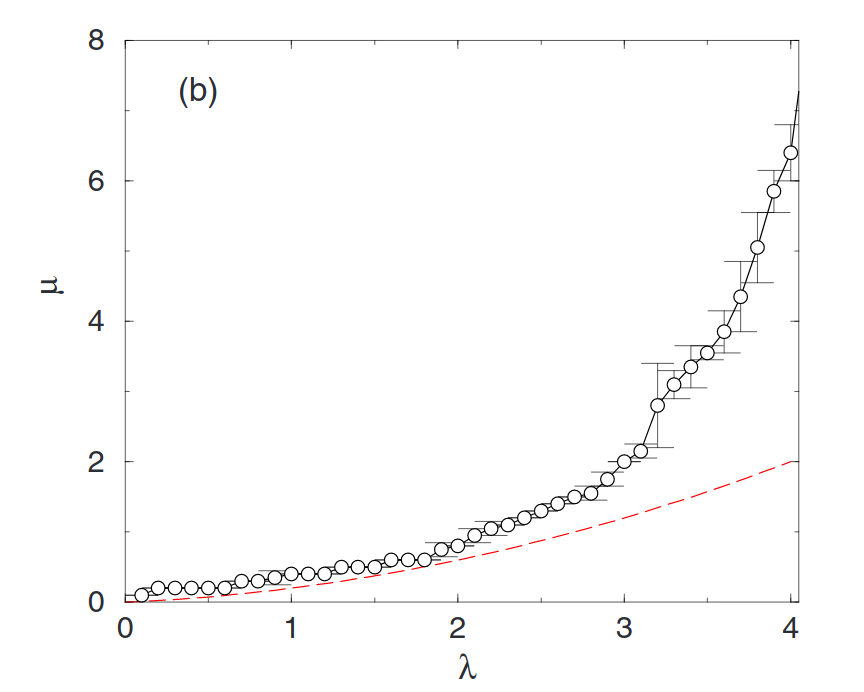
\includegraphics[width=14cm]{plots/6b.png}
%		\caption{Original Figure 6b}
	\end{subfigure}
	\begin{subfigure}{\linewidth}
		\centering
		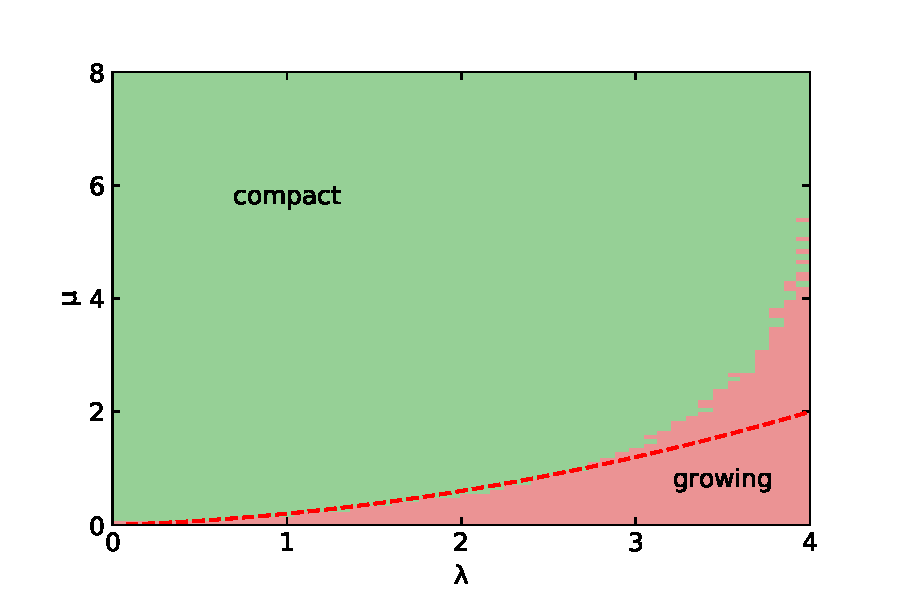
\includegraphics[width=15cm]{plots/6b.pdf}
%		\caption{Replicated Figure 6b}
	\end{subfigure}
	\caption{Phase Diagram for $p=0.1$}
\end{figure}

\clearpage
\section{Discussion}
\label{sec:disc}
The replicated versions of Figure 1 show similar behaviour to the original versions.\\

In Figure 5, it is clear that the probabilities in the replicated version is scaled by some value compared to the original. The replicated version is scaled so that the total probability is 1 (it is unclear why the authors of the original paper chose to apply this scaling). In addition to this, I do not observe the increase in simulated values before decreasing with respect to the theoretical prediction that the original paper had claimed.\\

Figure 6 deviates the most from the original paper. Instead of using the velocity of growth of the microtubule, I have used a simple threshold to determine whether the growth of a microtubule is bounded or not (microtubules that grow beyond a length of 5000 units after 100\,000 steps is deemed to be 'growing'). Such a method will underestimate the threshold value $\mu_\star$ given a $\lambda$ since slowly growing microtubules are deemed to be compact. However, this is a good first order approximation as the Figures above show.

\section{Acknowledgements}
This work has made use of \href{https://www.python.org}{Python} \citep{python}, and several Python packages: \href{https://www.numpy.org}{NumPy} \citep{harris2020array}, \href{https://www.matplotlib.org}{Matplotlib} \citep{hunter2007matplotlib} and \href{https://numba.pydata.org/}{Numba} \citep{lam2015numba}; as well as the IPython web application \href{https://jupyter.org/}{Jupyter} \citep{ipython}.

\bibliography{biblio}
\end{document}
